\documentclass{standalone}

\usepackage[english]{babel} % English language/hyphenation
\usepackage{clock} % Required for generation clock icon
\ClockFrametrue\ClockStyle=3 % Format the clock icons
\usepackage{gensymb} % gives the degree symbol
\usepackage{graphicx} % Required for including pictures
\usepackage{tikz} % Required for drawing custom shapes
\usetikzlibrary{arrows}
\usetikzlibrary{shapes.misc}
\usetikzlibrary{decorations.pathreplacing}

\begin{document}
	\def\glider#1#2#3{
		\begin{scope}[shift={#1}, rotate=#2, scale=#3]
			\fill[black](0,0) -- (1,0) -- (1,1) -- (0,1) -- cycle;
			\fill[black](8/7+0,0) -- (8/7+1,0) -- (8/7+1,1) -- (8/7+0,1) -- cycle;
			\fill[black](16/7+0,0) -- (16/7+1,0) -- (16/7+1,1) -- (16/7+0,1) -- cycle;
			\fill[black](16/7+0,8/7+0) -- (16/7+1,8/7+0) -- (16/7+1,8/7+1) -- (16/7+0,8/7+1) -- cycle;
			\fill[black](8/7+0,16/7+0) -- (8/7+1,16/7+0) -- (8/7+1,16/7+1) -- (8/7+0,16/7+1) -- cycle;
		\end{scope}
	}
	\def\lwss#1#2#3{
		\begin{scope}[shift={#1}, rotate=#2, scale=#3]
			\fill[black](0,0) -- (1,0) -- (1,1) -- (0,1) -- cycle;
			\fill[black](8/7+0,0) -- (8/7+1,0) -- (8/7+1,1) -- (8/7+0,1) -- cycle;
			\fill[black](16/7+0,0) -- (16/7+1,0) -- (16/7+1,1) -- (16/7+0,1) -- cycle;
			\fill[black](24/7+0,0) -- (24/7+1,0) -- (24/7+1,1) -- (24/7+0,1) -- cycle;
			\fill[black](32/7+0,8/7+0) -- (32/7+1,8/7+0) -- (32/7+1,8/7+1) -- (32/7+0,8/7+1) -- cycle;
			\fill[black](0,8/7+0) -- (1,8/7+0) -- (1,8/7+1) -- (0,8/7+1) -- cycle;
			\fill[black](0,16/7+0) -- (1,16/7+0) -- (1,16/7+1) -- (0,16/7+1) -- cycle;
			\fill[black](8/7+0,24/7+0) -- (8/7+1,24/7+0) -- (8/7+1,24/7+1) -- (8/7+0,24/7+1) -- cycle;
			\fill[black](32/7+0,24/7+0) -- (32/7+1,24/7+0) -- (32/7+1,24/7+1) -- (32/7+0,24/7+1) -- cycle;
		\end{scope}
	}
	\def\gggrake#1#2#3{
		\begin{scope}[shift={#1}, rotate=#2]
		% RAKES to MAKE row of GGGs
		\foreach \x in {1,...,4} \draw[thick,color=darkgray,-stealth] (10,-1.5+0.8*\x) -- (10+#3,-1.5+0.8*\x);
		\foreach \x in {1,...,4} \filldraw[color=black,fill=gray!50] (9,-1.7+0.8*\x) -- (10,-1.7+0.8*\x) -- (10,-1.3+0.8*\x) -- (9,-1.3+0.8*\x) -- cycle;
		
		% GLIDERS from RAKES to make GGGs
		\foreach \x in {1,2} \draw[thick,color=darkgray,-stealth] (8.71,-1.4+0.8*\x) -- (6.91 + 0.8*\x,0.4);
		\foreach \x in {3,4} \draw[thick,color=darkgray,-stealth] (8.71,-1.605+0.8*\x) -- (10.91 - 0.8*\x,0.595);
		\foreach \x in {1,2} \glider{(8.94,-1.37+0.8*\x)}{180}{0.08};
		\foreach \x in {3,4} \glider{(8.68,-1.37+0.8*\x)}{270}{0.08};
		\end{scope}
	}
	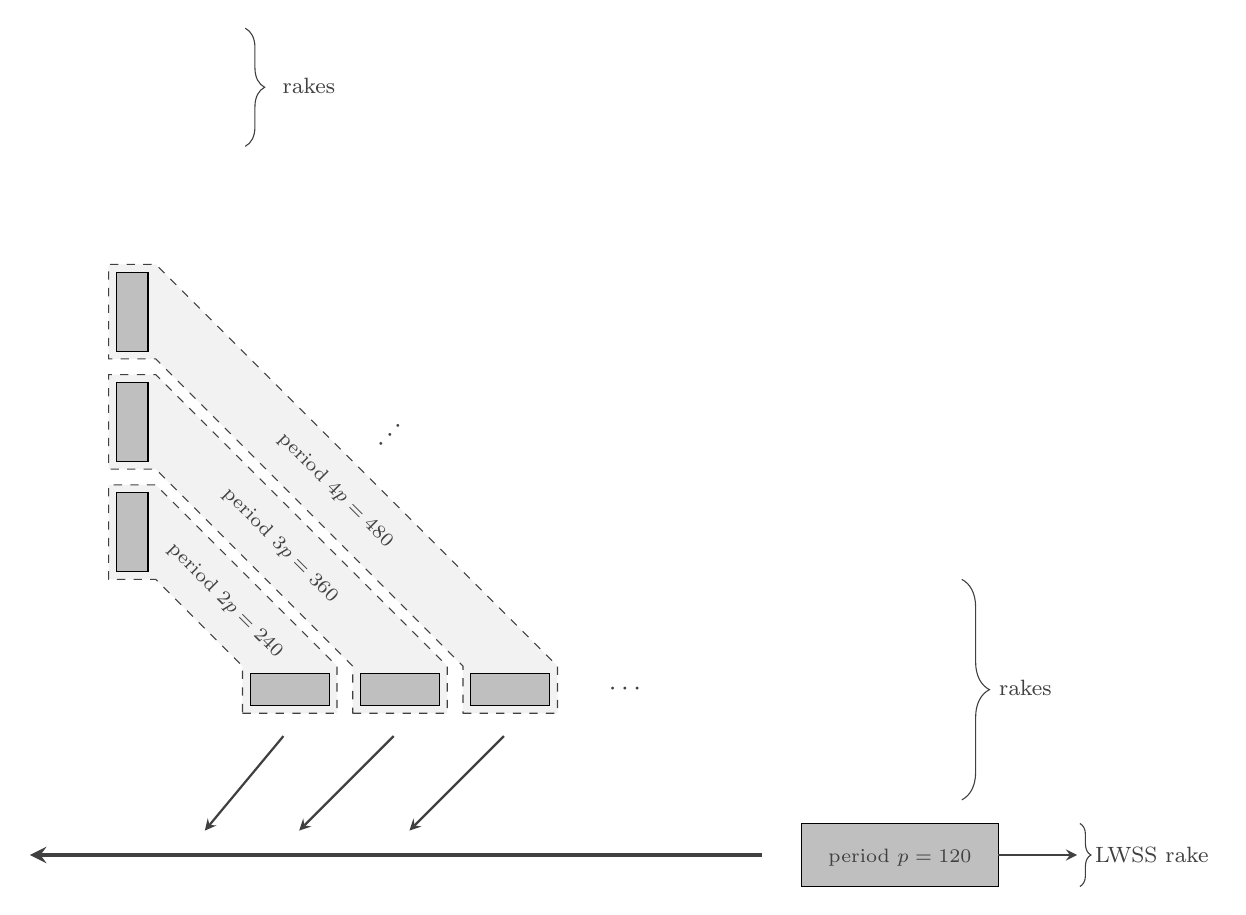
\begin{tikzpicture}%
		% DASHED GROUPINGS
		\filldraw[draw=darkgray,fill=gray!10,dashed] (0.9,0.2) -- (2.1,0.2) -- (2.1,0.8) -- (-0.2,3.1) -- (-0.8,3.1) -- (-0.8,1.9) -- (-0.2,1.9) -- (0.9,0.8) -- cycle;
		\draw[darkgray] (0.68,1.63) node[rotate=-45] {\scriptsize period~$2p = 240$};
		\filldraw[draw=darkgray,fill=gray!10,dashed] (2.3,0.2) -- (3.5,0.2) -- (3.5,0.8) -- (-0.2,4.5) -- (-0.8,4.5) -- (-0.8,3.3) -- (-0.2,3.3) -- (2.3,0.8) -- cycle;
		\draw[darkgray] (1.38,2.33) node[rotate=-45] {\scriptsize period~$3p = 360$};
		\filldraw[draw=darkgray,fill=gray!10,dashed] (3.7,0.2) -- (4.9,0.2) -- (4.9,0.8) -- (-0.2,5.9) -- (-0.8,5.9) -- (-0.8,4.7) -- (-0.2,4.7) -- (3.7,0.8) -- cycle;
		\draw[darkgray] (2.08,3.03) node[rotate=-45] {\scriptsize period~$4p = 480$};
		\draw[darkgray] (2.78,3.73) node[rotate=45] {$\cdots$};
			
		% UP-DOWN GUNS
		\filldraw[color=black,fill=gray!50] (-0.3,2) -- (-0.7,2) -- (-0.7,3) -- (-0.3,3) -- cycle;
		\filldraw[color=black,fill=gray!50] (-0.3,3.4) -- (-0.7,3.4) -- (-0.7,4.4) -- (-0.3,4.4) -- cycle;
		\filldraw[color=black,fill=gray!50] (-0.3,4.8) -- (-0.7,4.8) -- (-0.7,5.8) -- (-0.3,5.8) -- cycle;
	
		% LEFT-RIGHT GUNS
		\filldraw[color=black,fill=gray!50] (1,0.3) -- (2,0.3) -- (2,0.7) -- (1,0.7) -- cycle;
		\filldraw[color=black,fill=gray!50] (2.4,0.3) -- (3.4,0.3) -- (3.4,0.7) -- (2.4,0.7) -- cycle;
		\filldraw[color=black,fill=gray!50] (3.8,0.3) -- (4.8,0.3) -- (4.8,0.7) -- (3.8,0.7) -- cycle;
		\draw[darkgray] (5.758,0.5) node {$\cdots$};
		
		% GLIDERS from LEFT-RIGHT GUNS
		\draw[thick,color=darkgray,-stealth] (1.42,-0.09) -- (0.422,-1.29);
		\glider{(1.4,0.15)}{270}{0.08};
		\draw[thick,color=darkgray,-stealth] (2.82,-0.09) -- (1.62,-1.29);
		\glider{(2.8,0.15)}{270}{0.08};
		\draw[thick,color=darkgray,-stealth] (4.22,-0.09) -- (3.02,-1.29);
		\glider{(4.2,0.15)}{270}{0.08};
		
		% LWSS RAKE
		\filldraw[color=black,fill=gray!50] (8,-1.2) -- (10.5,-1.2) -- (10.5,-2) -- (8,-2) -- cycle;
		\draw[darkgray] (9.25,-2.13+0.5) node {\scriptsize period~$p=120$};
		\draw[thick,color=darkgray,-stealth] (10.5,-1.6) -- (11.5,-1.6);
		
		\draw[darkgray,decorate,decoration={brace,amplitude=4pt},xshift=1pt]
		(11.5,-1.2) --node [anchor=north,xshift=26pt,yshift=6.5pt]{\footnotesize LWSS rake} (11.5,-2);
		
		% LWSS from GUN
		\draw[ultra thick,color=darkgray,-stealth] (7.5,-1.6) -- (-1.8,-1.6);
		\lwss{(7.5,-2.23+0.5)}{0}{0.08};
		
		% RAKES to MAKE LEFT-RIGHT row of GGGs
		\gggrake{(-1,0)}{0}{1};
		\draw[darkgray,decorate,decoration={brace,amplitude=10pt},xshift=1pt]
		(10,1.9) --node [anchor=north,xshift=23pt,yshift=7pt]{\footnotesize rakes} (10,-0.9);
		
		% RAKES to MAKE UP-DOWN row of GGGs
		\gggrake{(0,-1.6)}{90}{0.5};
		\draw[darkgray,decorate,decoration={brace,amplitude=7pt},xshift=1pt]
		(0.9,8.9) --node [anchor=north,xshift=23pt,yshift=7pt]{\footnotesize rakes} (0.9,7.4);
	\end{tikzpicture}
\end{document}